\documentclass[11pt,a4paper]{article}

\usepackage[utf8]{inputenc}
\usepackage[margin=2.5cm]{geometry}
\usepackage{amsmath,amssymb,amsthm,mathtools,bm}
\usepackage{booktabs,array,enumitem}
\usepackage{tikz,pgfplots}
\pgfplotsset{compat=1.16}
\usetikzlibrary{arrows.meta,calc,positioning}
\usepackage[most]{tcolorbox}
\usepackage{float}
\usepackage[colorlinks=true,linkcolor=blue!50!black,urlcolor=blue!50!black]{hyperref}

\setlist{itemsep=2pt,topsep=4pt}

% ---------- macros ----------
\newcommand{\R}{\mathbb{R}}
\newcommand{\dd}{\mathrm{d}}
\newcommand{\LB}[2]{[#1,#2]}
\newcommand{\Dist}{\Delta}
\newcommand{\AccDist}{\Delta_A}
\newcommand{\dotq}{\dot q}
\DeclareMathOperator{\rank}{rank}
\DeclareMathOperator{\spn}{span}
\DeclareMathOperator{\Ker}{\mathcal{N}}

% ---------- theorem environments (amsthm) ----------
\theoremstyle{plain}
\newtheorem{theorem}{Theorem}[section]
\newtheorem{lemma}[theorem]{Lemma}
\newtheorem{proposition}[theorem]{Proposition}
\newtheorem{corollary}[theorem]{Corollary}
\theoremstyle{definition}
\newtheorem{definition}[theorem]{Definition}
\newtheorem{example}[theorem]{Example}
\newtheorem{algorithm}[theorem]{Algorithm}
\theoremstyle{remark}
\newtheorem*{remark}{Remark}

\tcbset{boxstyle/.style={enhanced,breakable,boxrule=0.5pt,arc=2pt,left=6pt,right=6pt,top=4pt,bottom=4pt,before skip=8pt,after skip=8pt}}
\tcolorboxenvironment{definition}{boxstyle,colback=green!4!white,colframe=green!40!black}
\tcolorboxenvironment{theorem}{boxstyle,colback=orange!6!white,colframe=orange!70!black}
\tcolorboxenvironment{lemma}{boxstyle,colback=orange!6!white,colframe=orange!70!black}
\tcolorboxenvironment{proposition}{boxstyle,colback=orange!6!white,colframe=orange!70!black}
\tcolorboxenvironment{corollary}{boxstyle,colback=orange!6!white,colframe=orange!70!black}
\tcolorboxenvironment{example}{boxstyle,colback=gray!6!white,colframe=gray!60!black}
\tcolorboxenvironment{algorithm}{boxstyle,colback=violet!5!white,colframe=violet!60!black}

% Blue "Intuition" box
\newtcolorbox{intuition}{enhanced,breakable,colback=blue!5!white,colframe=blue!60!black,
  boxrule=0.5pt,arc=2pt,fonttitle=\bfseries,title=Intuition,
  before skip=8pt,after skip=10pt}

% wheel drawing helper: \wheel{(center)}{angle}{color}
\newcommand{\wheel}[3]{\begin{scope}[shift={#1},rotate=#2]
  \draw[fill=#3,rounded corners=1pt] (-0.4,-0.12) rectangle (0.4,0.12);\end{scope}}

\title{\textbf{Autonomous and Mobile Robotics}\\[2pt]
\large Lecture 4 --- Bicycle Kinematics and Nonlinear Controllability\\[2pt]
\normalsize (Lie brackets and Chow's theorem)}
\author{Autonomous and Mobile Robotics, Sapienza (prof.\ G.\ Oriolo)}
\date{}

\emergencystretch=3em
\begin{document}
\maketitle
\tableofcontents
\bigskip

\noindent\textbf{Conventions.} The driving and steering inputs are written $u_1,u_2$ (for the unicycle also $v,\omega$). The Lie bracket is defined as
$\LB{g_1}{g_2}=\frac{\partial g_2}{\partial q}g_1-\frac{\partial g_1}{\partial q}g_2$.
$\LB{g_1}{g_2}=\frac{\partial g_2}{\partial q}g_1-\frac{\partial g_1}{\partial q}g_2$.

% =====================================================================
\section{Recap: kinematic models and the unicycle}

\begin{definition}[Kinematic model]
Let a wheeled robot with configuration $q\in\R^n$ be subject to $k$ independent Pfaffian (kinematic) constraints
\[
A(q)\,\dot q=0,\qquad A(q)\in\R^{k\times n}.
\]
Admissible velocities are exactly $\dot q\in\Ker(A(q))$, a subspace of dimension $m=n-k$. Choosing a basis $g_1(q),\dots,g_m(q)$ of the null space gives the \emph{kinematic model}
\[
\dot q=\sum_{i=1}^{m} g_i(q)\,u_i .
\]
\end{definition}

\begin{example}[Unicycle]
With $q=(x,y,\theta)$ the single pure-rolling constraint is $\sin\theta\,\dot x-\cos\theta\,\dot y=0$, and
\[
\dot q=\underbrace{\begin{pmatrix}\cos\theta\\ \sin\theta\\ 0\end{pmatrix}}_{\text{drive VF } g_1}v
+\underbrace{\begin{pmatrix}0\\0\\1\end{pmatrix}}_{\text{steer VF } g_2}\omega .
\]
\end{example}

\begin{intuition}
The two vector fields are the two ``elementary motions'' of the robot: $g_1$ rolls it along its heading without changing the heading, $g_2$ spins it in place. Every admissible velocity is a mix of the two. Example: at $\theta=\pi/4$ with $v=1$, $\omega=0$ the robot moves with $\dot q=(0.71,0.71,0)^T$, a straight diagonal line. We have $n=3$ coordinates but only $m=2$ inputs: the missing direction (sideways) is exactly what is forbidden by the constraint.
\end{intuition}

% =====================================================================
\section{The bicycle model}

\subsection{Configuration and constraints}

The bicycle has a fixed rear wheel and a steerable front wheel. Let $(x,y)$ be the rear-wheel contact point, $\theta$ the orientation of the body, $\phi$ the steering angle, $\ell$ the wheelbase, and $(x_f,y_f)$ the front-wheel contact point:
\[
q=\begin{pmatrix}x\\y\\\theta\\\phi\end{pmatrix},\qquad
\mathcal C=\R^2\times SO(2)\times SO(2),\qquad n=4 .
\]
Both wheels roll without lateral slipping:
\begin{align}
\sin\theta\,\dot x-\cos\theta\,\dot y&=0 &&\text{(pure rolling, rear wheel)}\tag{R}\\
\sin(\theta+\phi)\,\dot x_f-\cos(\theta+\phi)\,\dot y_f&=0 &&\text{(pure rolling, front wheel)}\tag{F}
\end{align}

\begin{figure}[H]
\centering
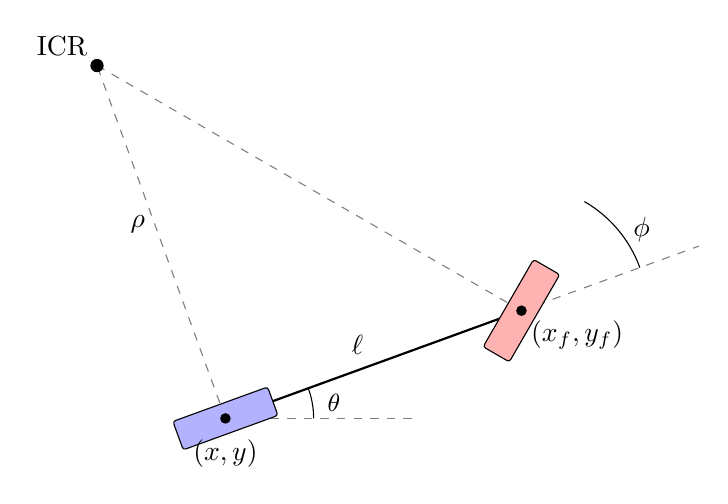
\begin{tikzpicture}[>=Stealth,scale=1.6]
\coordinate (R) at (0,0);
\coordinate (F) at (2.349,0.855);
\coordinate (I) at (-1.019,2.800);
\draw[dashed,gray] (R)--(I) node[pos=0.55,left,black]{$\rho$};
\draw[dashed,gray] (F)--(I);
\draw[dashed,gray] (-0.3,0)--(1.5,0);
\draw[dashed,gray] (F)--++(20:1.5);
\draw[thick] (R)--(F) node[midway,above left]{$\ell$};
\wheel{(R)}{20}{blue!30}
\wheel{(F)}{60}{red!30}
\fill (I) circle (1.5pt) node[above left]{ICR};
\fill (R) circle (1.2pt) node[below,yshift=-4pt]{$(x,y)$};
\fill (F) circle (1.2pt) node[below right]{$(x_f,y_f)$};
\draw (0.7,0) arc(0:20:0.7) node[midway,right,xshift=2pt]{\small$\theta$};
\draw[shift={(F)}] (20:1.0) arc(20:60:1.0) node[midway,right,xshift=2pt]{$\phi$};
\end{tikzpicture}
\caption{Bicycle geometry. The axes of the two wheels (perpendicular to the rolling directions) meet at the instantaneous centre of rotation (ICR); the whole robot rotates instantaneously about it, with turning radius $\rho=\ell/\tan\phi$.}
\label{fig:bicycle}
\end{figure}

\begin{intuition}
At every instant a rigid body that moves in the plane is rotating about a single point, the ICR. A rolling wheel can only move perpendicular to its axle, so the ICR must lie on the line through the axle. With two wheels, the ICR is the intersection of the two axle lines (Fig.~\ref{fig:bicycle}) and \emph{all} points of the robot contribute to this one rotation. Numbers: for $\ell=1$ and $\phi=30^\circ$ the radius is $\rho=1/\tan30^\circ\approx1.73$; as $\phi\to0$ the axle lines become parallel and the ICR escapes to infinity (straight motion).
\end{intuition}

\subsection{Writing the front constraint with rear-wheel coordinates}

\begin{lemma}[Front-wheel constraint]
\label{lem:front}
Constraint (F) is equivalent to
\[
\sin(\theta+\phi)\,\dot x-\cos(\theta+\phi)\,\dot y-\ell\cos\phi\,\dot\theta=0 .
\]
\end{lemma}
\begin{proof}
The front contact point is $x_f=x+\ell\cos\theta$, $y_f=y+\ell\sin\theta$, hence
\[
\dot x_f=\dot x-\ell\sin\theta\,\dot\theta,\qquad \dot y_f=\dot y+\ell\cos\theta\,\dot\theta .
\]
Substituting in (F):
\[
\sin(\theta+\phi)\dot x-\cos(\theta+\phi)\dot y-\ell\dot\theta\big[\sin(\theta+\phi)\sin\theta+\cos(\theta+\phi)\cos\theta\big]=0,
\]
and the bracket equals $\cos\big((\theta+\phi)-\theta\big)=\cos\phi$.
\end{proof}

\begin{proposition}[Constraint matrix]
With $k=2$ constraints, $A(q)\dot q=0$ where
\[
A(q)=\begin{pmatrix}
\sin\theta & -\cos\theta & 0 & 0\\
\sin(\theta+\phi) & -\cos(\theta+\phi) & -\ell\cos\phi & 0
\end{pmatrix}.
\]
Hence $\dim\Ker(A(q))=n-k=2$ and two linearly independent vector fields are needed.
\end{proposition}

\subsection{Rear-wheel drive (RWD) kinematic model}

\begin{proposition}[RWD bicycle]
\label{prop:rwd}
A basis of $\Ker(A(q))$ is
\[
g_1(q)=\begin{pmatrix}\cos\theta\\ \sin\theta\\ \frac1\ell\tan\phi\\ 0\end{pmatrix},\qquad
g_2(q)=\begin{pmatrix}0\\0\\0\\1\end{pmatrix},
\]
so that
\[
\dot q=\begin{pmatrix}\dot x\\\dot y\\\dot\theta\\\dot\phi\end{pmatrix}
=\begin{pmatrix}\cos\theta\\ \sin\theta\\ \frac1\ell\tan\phi\\ 0\end{pmatrix}u_1
+\begin{pmatrix}0\\0\\0\\1\end{pmatrix}u_2,
\qquad u_1=\pm\sqrt{\dot x^2+\dot y^2},\quad u_2=\dot\phi .
\]
\end{proposition}
\begin{proof}
$g_2\in\Ker(A)$ trivially, because the last column of $A$ is zero. For $g_1$ take $(\cos\theta,\sin\theta,\alpha,0)^T$; the first row gives $\sin\theta\cos\theta-\cos\theta\sin\theta=0$ for any $\alpha$, and the second gives
\[
\sin(\theta+\phi)\cos\theta-\cos(\theta+\phi)\sin\theta-\ell\cos\phi\,\alpha=\sin\phi-\ell\cos\phi\,\alpha=0
\;\Longrightarrow\;\alpha=\tfrac1\ell\tan\phi .
\]
Finally $\dot x^2+\dot y^2=(\cos^2\theta+\sin^2\theta)u_1^2=u_1^2$, so $u_1$ is the driving speed of the rear wheel, and $u_2=\dot\phi$ is the steering velocity.
\end{proof}

\begin{intuition}
Think of the rear wheel as the ``engine'' and the front wheel as just a rudder. The rear point moves along the heading with speed $u_1$ (first two components of $g_1$), while the heading changes at the rate $\dot\theta=\frac{u_1}{\ell}\tan\phi=u_1/\rho$: exactly the angular rate of a point travelling at speed $u_1$ on a circle of radius $\rho=\ell/\tan\phi$. The steering vector field $g_2$ only turns the handlebar. Numbers: $\ell=1$, $\phi=30^\circ$, $u_1=1$ gives $\dot\theta\approx0.58$ rad/s.
\end{intuition}

\paragraph{Validity and singularity.} The model is good \emph{if the bicycle is rear-wheel drive}. At $\phi=\pi/2$ the vector field $g_1$ ``blows up'' ($\tan\phi\to\infty$): a singularity. Physically, with the front wheel perpendicular to the body, a nonzero rear speed $v\neq0$ would require the front wheel to \emph{slip} sideways, which the pure-rolling hypothesis excludes.

% =====================================================================
\section{The front-wheel drive case}

For a front-wheel-drive (FWD) vehicle the natural control is the speed of the front wheel, $u_1=\pm\sqrt{\dot x_f^2+\dot y_f^2}$.

\begin{proposition}[FWD bicycle]
Rescaling $g_1\mapsto g_1\cos\phi$ and keeping $g_2$,
\[
\dot q=\begin{pmatrix}\cos\theta\cos\phi\\ \sin\theta\cos\phi\\ \frac1\ell\sin\phi\\ 0\end{pmatrix}u_1+\begin{pmatrix}0\\0\\0\\1\end{pmatrix}u_2,
\qquad \dot x_f^2+\dot y_f^2=u_1^2,\quad u_2=\dot\phi .
\]
\end{proposition}
\begin{proof}
From $\dot x_f=\dot x-\ell\sin\theta\,\dot\theta$ and $\dot y_f=\dot y+\ell\cos\theta\,\dot\theta$ we get
\[
\dot x_f=u_1(\cos\theta\cos\phi-\sin\theta\sin\phi)=u_1\cos(\theta+\phi),\qquad
\dot y_f=u_1\sin(\theta+\phi),
\]
so $\dot x_f^2+\dot y_f^2=u_1^2$. Since $\cos\phi\,g_1\in\Ker(A)$ and $g_2\in\Ker(A)$, this is still a basis of the null space wherever $\cos\phi\ne0$, and the rescaled field is also valid (smooth, nonzero) at $\phi=\pi/2$.
\end{proof}

\begin{figure}[H]
\centering
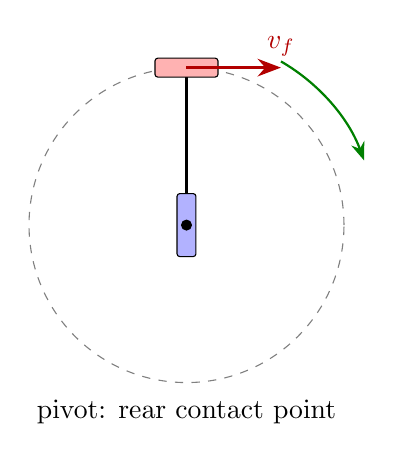
\begin{tikzpicture}[>=Stealth]
\coordinate (R) at (0,0);
\coordinate (F) at (0,2);
\draw[dashed,gray] (R) circle (2);
\draw[thick] (R)--(F);
\wheel{(R)}{90}{blue!30}
\wheel{(F)}{0}{red!30}
\fill (R) circle (2pt);
\draw[->,very thick,red!70!black] (F)--++(1.2,0) node[above]{$v_f$};
\draw[->,thick,green!50!black] (60:2.4) arc(60:20:2.4);
\node[below] at (0,-2.1) {pivot: rear contact point};
\end{tikzpicture}
\caption{FWD bicycle at $\phi=\pi/2$: the front wheel pushes the vehicle sideways and it pivots about the rear-wheel contact point.}
\label{fig:pivot}
\end{figure}

\begin{intuition}
If you \emph{drive} the front wheel you can steer it all the way to $\phi=\pi/2$ and still move: the front wheel rolls in its own direction, perpendicular to the body, and the body simply rotates about the rear contact point (Fig.~\ref{fig:pivot}) with $\dot\theta=u_1/\ell$. So you can move in circle around the rear point \emph{without hitting any singularity}. In the RWD model the same configuration would require infinite $\dot\theta$ per unit of rear speed.
\end{intuition}

% =====================================================================
\section{Controllability}

\subsection{Is there a universal manoeuvre?}

\begin{algorithm}[Universal manoeuvre for the bicycle]
To go from $q_i$ to any $q_f$:
\begin{enumerate}[label=(\arabic*)]
\item use the ICR: with the wheel steered, drive along a circle until the heading points towards the goal;
\item steer the wheel back to straight;
\item go straight along a line, then finish with another circular arc to match the final heading and steering.
\end{enumerate}
\end{algorithm}

\begin{figure}[H]
\centering
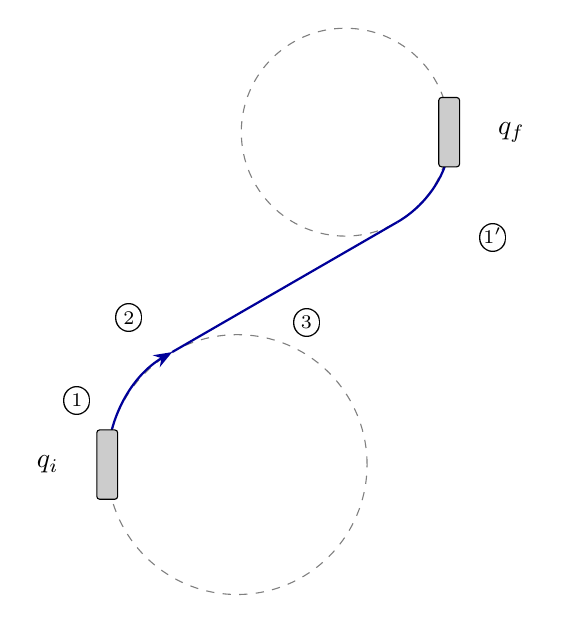
\begin{tikzpicture}[>=Stealth,scale=1.1]
\draw[dashed,gray] (1.5,0) circle (1.5);
\draw[dashed,gray] (2.748,3.838) circle (1.2);
\draw[thick,blue!60!black,->] (1.5,0)+(180:1.5) arc(180:120:1.5);
\draw[thick,blue!60!black] (0.75,1.299)--(3.348,2.799);
\draw[thick,blue!60!black,->] (2.748,3.838)+(-60:1.2) arc(-60:0:1.2);
\wheel{(0,0)}{90}{gray!40}
\wheel{(3.948,3.838)}{90}{gray!40}
\node[left] at (-0.45,0) {$q_i$};
\node[right] at (4.4,3.838) {$q_f$};
\node at (-0.35,0.7) {\textcircled{\scriptsize1}};
\node at (0.25,1.65) {\textcircled{\scriptsize2}};
\node at (2.3,1.6) {\textcircled{\scriptsize3}};
\node at (4.45,2.6) {\textcircled{\scriptsize$1'$}};
\end{tikzpicture}
\caption{Schematic universal manoeuvre (arc around an ICR, straight line, arc). The numbers refer to the steps of the algorithm; $1'$ is the final arc that matches the target heading.}
\end{figure}

\begin{intuition}
It is the same idea as parking: any pose can be reached by combining only two primitives, rotating about an ICR and driving straight. Hence, although the bicycle has only two inputs for four configuration variables, \emph{it can reach every configuration}. This is possible precisely because the velocity constraints are \emph{non-integrable} (nonholonomic): if they were integrable, the robot would be confined to a lower-dimensional surface of $\mathcal C$ and could not reach everything.
\end{intuition}

\subsection{Nonlinear controllability}

We study driftless nonlinear systems
\[
\dot x=\sum_{i=1}^m g_i(x)u_i,\qquad x\in\R^n,\; u\in\R^m,
\]
(``driftless'': no term independent of $u$; for us $x$ is the configuration $q$).

\begin{definition}[Controllability]
The system is \emph{controllable} if, for any pair $(x_i,x_f)$, there exist $T>0$ and an input $u(t)$, $t\in[0,T]$, such that the trajectory starting at $x(0)=x_i$ satisfies $x(T)=x_f$.
\end{definition}

% =====================================================================
\section{The Lie bracket}

\begin{definition}[Lie bracket]
Let $g_1,g_2$ be two vector fields on $\R^n$. The vector field
\[
\LB{g_1}{g_2}(x)=\frac{\partial g_2}{\partial x}\,g_1(x)-\frac{\partial g_1}{\partial x}\,g_2(x)
\]
(where $\partial g_i/\partial x$ is the Jacobian) is the \emph{Lie bracket} (LB) of $g_1,g_2$.
\end{definition}

Immediate properties: $\LB{g_1}{g_2}=-\LB{g_2}{g_1}$ (hence $\LB{g}{g}=0$), and $\LB{g_1}{g_2}=0$ for constant fields.

\begin{example}[A bracket in $\R^3$]
\label{ex:lb3}
Let $g_1=(\cos x_3,\sin x_3,0)^T$ and $g_2=(0,0,x_1)^T$. Then
\begin{align*}
\LB{g_1}{g_2}(x)&=
\underbrace{\begin{pmatrix}0&0&0\\0&0&0\\1&0&0\end{pmatrix}}_{\partial g_2/\partial x}\begin{pmatrix}\cos x_3\\\sin x_3\\0\end{pmatrix}
-\underbrace{\begin{pmatrix}0&0&-\sin x_3\\0&0&\cos x_3\\0&0&0\end{pmatrix}}_{\partial g_1/\partial x}\begin{pmatrix}0\\0\\x_1\end{pmatrix}\\
&=\begin{pmatrix}0\\0\\\cos x_3\end{pmatrix}-\begin{pmatrix}-x_1\sin x_3\\x_1\cos x_3\\0\end{pmatrix}
=\begin{pmatrix}x_1\sin x_3\\-x_1\cos x_3\\\cos x_3\end{pmatrix}.
\end{align*}
This is a \emph{new} vector field which, in this case, is linearly independent of $g_1,g_2$ (the determinant of $[g_1\ g_2\ \LB{g_1}{g_2}]$ is $x_1^2$, nonzero for $x_1\neq0$).
\end{example}

\begin{intuition}
The bracket measures \emph{how much the flows of two vector fields fail to commute}: moving first along $g_1$ then $g_2$ ends in a different place than $g_2$ then $g_1$. The difference of the two endpoints is (to second order) the bracket. If the bracket points in a direction that $g_1,g_2$ cannot generate directly, then ``wiggling'' between the two fields gives access to new directions of motion, which is the key to controllability.
\end{intuition}

% =====================================================================
\section{Interpretation of the Lie bracket}

Consider the 2-input system $\dot x=g_1(x)u_1+g_2(x)u_2$ and the piecewise-constant input of duration $4\varepsilon$.

\begin{algorithm}[Lie-bracket manoeuvre]
\label{alg:lb}
\[
(u_1,u_2)=\begin{cases}
(1,0)&t\in[0,\varepsilon)\\
(0,1)&t\in[\varepsilon,2\varepsilon)\\
(-1,0)&t\in[2\varepsilon,3\varepsilon)\\
(0,-1)&t\in[3\varepsilon,4\varepsilon).
\end{cases}
\]
\end{algorithm}

\begin{figure}[H]
\centering
\begin{tikzpicture}[x=1.4cm,y=0.9cm,>=Stealth]
\draw[->] (0,0)--(4.7,0) node[right]{$t$};
\draw[->] (0,-1.4)--(0,1.4) node[above]{$u_1$};
\draw[thick,blue!70!black] (0,1)--(1,1)--(1,0)--(2,0)--(2,-1)--(3,-1)--(3,0)--(4,0);
\draw[->] (0,-4.4)--(4.7,-4.4) node[right]{$t$};
\draw[->] (0,-5.8)--(0,-3.0) node[above]{$u_2$};
\draw[thick,red!70!black] (0,-4.4)--(1,-4.4)--(1,-3.4)--(2,-3.4)--(2,-4.4)--(3,-4.4)--(3,-5.4)--(4,-5.4)--(4,-4.4);
\foreach \i/\l in {1/\varepsilon,2/2\varepsilon,3/3\varepsilon,4/4\varepsilon}{
  \draw[gray,dotted] (\i,1.2)--(\i,-5.6);
  \node[font=\scriptsize,fill=white,inner sep=1pt] at (\i,0.3) {$\l$};
  \node[font=\scriptsize,fill=white,inner sep=1pt] at (\i,-4.1) {$\l$};
}
\node[left,font=\scriptsize] at (0,1) {$1$};
\node[left,font=\scriptsize] at (0,-1) {$-1$};
\node[left,font=\scriptsize] at (0,-3.4) {$1$};
\node[left,font=\scriptsize] at (0,-5.4) {$-1$};
\end{tikzpicture}
\caption{Control sequence of Algorithm~\ref{alg:lb}: forward $g_1$, forward $g_2$, backward $g_1$, backward $g_2$.}
\end{figure}

\begin{proposition}[Displacement of the LB manoeuvre]
\label{prop:lbdisp}
Starting from $x(0)=x_0$, the state after the sequence of Algorithm~\ref{alg:lb} is
\[
x(4\varepsilon)=x(0)+\varepsilon^2\,\LB{g_1}{g_2}(x_0)+O(\varepsilon^3),
\]
where the remainder goes to zero as $\varepsilon^3$ or faster when $\varepsilon\to0$.
\end{proposition}
\begin{proof}
Write $a=g_1(x_0)$, $b=g_2(x_0)$, $A=\partial g_1/\partial x(x_0)$, $B=\partial g_2/\partial x(x_0)$. The flow of a field $g$ for time $t$ is $x+t\,g(x)+\tfrac{t^2}{2}\tfrac{\partial g}{\partial x}g(x)+O(t^3)$. Applying the four phases in turn, up to terms $O(\varepsilon^2)$:
\begin{align*}
x_1&=x_0+\varepsilon a+\tfrac{\varepsilon^2}{2}Aa,\\
x_2&=x_1+\varepsilon g_2(x_1)+\tfrac{\varepsilon^2}2Bb=x_0+\varepsilon(a+b)+\varepsilon^2\big(\tfrac12Aa+Ba+\tfrac12Bb\big),\\
x_3&=x_2-\varepsilon g_1(x_2)+\tfrac{\varepsilon^2}2Aa=x_0+\varepsilon b+\varepsilon^2\big(Ba+\tfrac12Bb-Ab\big),
\end{align*}
using $g_1(x_2)=a+\varepsilon A(a+b)+O(\varepsilon^2)$. Finally $g_2(x_3)=b+\varepsilon Bb+O(\varepsilon^2)$ and
\[
x_4=x_3-\varepsilon g_2(x_3)+\tfrac{\varepsilon^2}2Bb=x_0+\varepsilon^2(Ba-Ab)+O(\varepsilon^3)
=x_0+\varepsilon^2\LB{g_1}{g_2}(x_0)+O(\varepsilon^3).\qedhere
\]
\end{proof}

\begin{figure}[H]
\centering
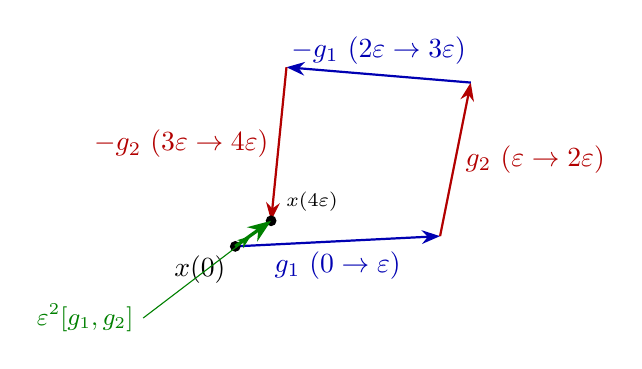
\begin{tikzpicture}[>=Stealth,scale=1.3]
\coordinate (P0) at (0,0);
\coordinate (P1) at (2,0.1);
\coordinate (P2) at (2.3,1.6);
\coordinate (P3) at (0.5,1.75);
\coordinate (P4) at (0.35,0.25);
\draw[thick,blue!70!black,->] (P0)--(P1) node[midway,below]{$g_1$ ($0\to\varepsilon$)};
\draw[thick,red!70!black,->] (P1)--(P2) node[midway,right]{$g_2$ ($\varepsilon\to2\varepsilon$)};
\draw[thick,blue!70!black,->] (P2)--(P3) node[midway,above]{$-g_1$ ($2\varepsilon\to3\varepsilon$)};
\draw[thick,red!70!black,->] (P3)--(P4) node[midway,left]{$-g_2$ ($3\varepsilon\to4\varepsilon$)};
\fill (P0) circle (1.5pt) node[below left]{$x(0)$};
\fill (P4) circle (1.5pt);
\node[above right,font=\scriptsize,xshift=2pt] at (P4) {$x(4\varepsilon)$};
\draw[very thick,green!50!black,->] (P0)--(P4);
\draw[green!50!black,->] (-0.9,-0.7) node[left]{\small $\varepsilon^2\LB{g_1}{g_2}$} -- (0.15,0.1);
\end{tikzpicture}
\caption{The four legs of the manoeuvre almost close a loop; the gap is the displacement $\varepsilon^2\LB{g_1}{g_2}(x_0)$ (schematic, exaggerated).}
\label{fig:lbloop}
\end{figure}

\begin{intuition}
Going forward-sideways-backward-sideways ``almost'' returns to the start, like the parking manoeuvre. The residual gap is second order in the time, $\varepsilon^2$, and is the Lie bracket. Unicycle check ($\theta=0$): go forward $\varepsilon$, rotate by $+\varepsilon$, go backward $\varepsilon$ along the rotated heading, rotate back. The net motion in $y$ is $-\varepsilon\sin\varepsilon\approx-\varepsilon^2$, i.e.\ a sideways shift, exactly $\varepsilon^2\LB{g_1}{g_2}=\varepsilon^2(\sin\theta,-\cos\theta,0)=\varepsilon^2(0,-1,0)$, even though the unicycle cannot move sideways directly. Numbers: with $\varepsilon=0.1$ the path costs $4\varepsilon=0.4$ time units but moves only $\varepsilon^2=0.01$ sideways: bracket motions are cheap in inputs but slow.
\end{intuition}

% =====================================================================
\section{Distributions, accessibility and Chow's theorem}

\begin{definition}[Input distribution]
For $\dot x=\sum_{i=1}^m g_i(x)u_i$ the \emph{input distribution} $\Dist=\{g_1(x),\dots,g_m(x)\}$ associates to each $x$ the subspace $\spn\{g_1(x),\dots,g_m(x)\}$ (all directions in which the inputs can push directly).
\end{definition}

\begin{definition}[Accessibility distribution]
The \emph{accessibility distribution} $\AccDist$ is the distribution generated by the input fields and all their iterated brackets:
\[
\AccDist=\Big\{g_1,\dots,g_m,\ \dots,\LB{g_i}{g_j},\ \dots,\ \LB{g_i}{\LB{g_j}{g_k}},\ \dots\Big\},
\]
with all 1st-order brackets, all 2nd-order brackets, and so on.
\end{definition}

\begin{theorem}[Chow]
\label{thm:chow}
Consider the driftless system $\dot x=\sum_i g_i(x)u_i$ on $\R^n$ and assume $\dim\AccDist(x)$ is constant for all $x$. Then the system is controllable if and only if
\[
\dim\AccDist=n .
\]
\end{theorem}

\begin{remark}
This result is known as \emph{Chow's theorem}, the \emph{Lie algebra rank condition} or the \emph{accessibility rank condition}. In practice, for low-order brackets one computes
\[
\rank\Big(g_1\ \ g_m\ \cdots\ \LB{g_i}{g_j}\ \cdots\ \LB{g_i}{\LB{g_j}{g_k}}\ \cdots\Big)=n,
\]
adding brackets of increasing order until the rank reaches $n$ (or no new independent direction appears).
\end{remark}

\begin{intuition}
The inputs give you $m$ directions for free. Each bracket manoeuvre buys you one more direction (Prop.~\ref{prop:lbdisp}), brackets of brackets buy yet more. If after collecting all of them the directions span the whole state space, there is no direction in which you are stuck, so you can steer anywhere. Analogy: you can only drive a car forward/backward and turn, yet by combining these ($\to$ parallel parking) you effectively obtain a ``slide sideways'' control.
\end{intuition}

% =====================================================================
\section{Application to the unicycle}

\begin{example}[Controllability of the unicycle]
With $q=(x,y,\theta)^T$, $g_1=(\cos\theta,\sin\theta,0)^T$ (drive) and $g_2=(0,0,1)^T$ (steer):
\[
\LB{g_1}{g_2}(q)=\underbrace{0}_{\partial g_2/\partial q=0}\cdot g_1-\begin{pmatrix}0&0&-\sin\theta\\0&0&\cos\theta\\0&0&0\end{pmatrix}\begin{pmatrix}0\\0\\1\end{pmatrix}
=\begin{pmatrix}\sin\theta\\-\cos\theta\\0\end{pmatrix}=:g_3(q),
\]
and
\[
\rank\begin{pmatrix}\cos\theta&0&\sin\theta\\\sin\theta&0&-\cos\theta\\0&1&0\end{pmatrix}=3=n .
\]
(The determinant is $1$ for all $\theta$.)
\end{example}

\begin{corollary}
The unicycle is controllable by Theorem~\ref{thm:chow}.
\end{corollary}

\begin{figure}[H]
\centering
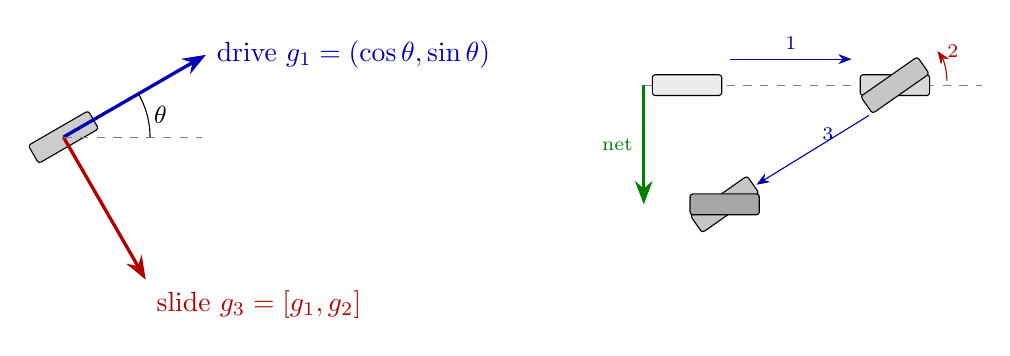
\begin{tikzpicture}[>=Stealth,scale=1.1]
\begin{scope}
\wheel{(0,0)}{30}{gray!40}
\draw[->,very thick,blue!70!black] (0,0)--(30:1.9) node[right]{drive $g_1=(\cos\theta,\sin\theta)$};
\draw[->,very thick,red!70!black] (0,0)--(-60:1.9) node[below right]{slide $g_3=\LB{g_1}{g_2}$};
\draw[dashed,gray] (0,0)--(1.6,0);
\draw (1.0,0) arc(0:30:1.0) node[midway,right,xshift=-1pt]{\small$\theta$};
\end{scope}
\begin{scope}[xshift=7.2cm,yshift=0.6cm]
\draw[gray,dashed] (-0.5,0)--(3.4,0);
\wheel{(0,0)}{0}{gray!15}
\wheel{(2.4,0)}{0}{gray!30}
\wheel{(2.4,0)}{35}{gray!45}
\wheel{(0.434,-1.376)}{35}{gray!45}
\wheel{(0.434,-1.376)}{0}{gray!70}
\draw[->,blue!70!black] (0.5,0.3)--(1.9,0.3) node[above,midway,font=\scriptsize]{1};
\draw[->,red!70!black] (3.0,0.05) arc(0:35:0.6) node[right,font=\scriptsize]{2};
\draw[->,blue!70!black] (2.1,-0.35)--(0.8,-1.15) node[midway,above right,font=\scriptsize]{3};
\draw[->,green!50!black,very thick] (-0.5,0)--(-0.5,-1.376) node[midway,left,font=\scriptsize]{net};
\end{scope}
\end{tikzpicture}
\caption{Left: drive and slide vectors of the unicycle. Right: LB manoeuvre (1 forward, 2 rotate, 3 backward, then rotate back): the net displacement is sideways (angles exaggerated).}
\end{figure}

\begin{intuition}
The new vector field $g_3=\LB{g_1}{g_2}$ points perpendicular to the heading: it is the \emph{slide} that the wheel forbids. Together $g_1$ (drive), $g_2$ (steer) and $g_3$ (slide) span all of $\R^3$ at every configuration, so the unicycle can reach every $(x,y,\theta)$.
\end{intuition}

% =====================================================================
\section{Application to the bicycle}

Take the RWD bicycle ($n=4$)
\[
\dot q=\begin{pmatrix}\cos\theta\\\sin\theta\\\tan\phi/\ell\\0\end{pmatrix}v+\begin{pmatrix}0\\0\\0\\1\end{pmatrix}\omega .
\]
The same computation applies to the FWD model. Since $n=4$ and only two inputs are available, we need the brackets up to the second order.

\begin{proposition}[Brackets of the bicycle]
\label{prop:bicyclebr}
With $g_1,g_2$ as above,
\begin{align*}
\LB{g_1}{g_2}&=-\frac{\partial g_1}{\partial\phi}=\begin{pmatrix}0\\0\\-\dfrac{1}{\ell\cos^2\phi}\\0\end{pmatrix},\\
\LB{g_1}{\LB{g_1}{g_2}}&=\begin{pmatrix}-\dfrac{\sin\theta}{\ell\cos^2\phi}\\[6pt]\dfrac{\cos\theta}{\ell\cos^2\phi}\\0\\0\end{pmatrix}.
\end{align*}
\end{proposition}
\begin{proof}
Only $g_1$ depends on $\phi$, and $g_2=\partial/\partial\phi$ is constant, so $\LB{g_1}{g_2}=-\frac{\partial g_1}{\partial q}g_2=-\frac{\partial g_1}{\partial\phi}=-(0,0,\frac{1}{\ell\cos^2\phi},0)^T$. Let $w=\LB{g_1}{g_2}=(0,0,-\sigma,0)^T$ with $\sigma=1/(\ell\cos^2\phi)$. Then $\frac{\partial w}{\partial q}g_1=0$ (since $w$ depends only on $\phi$ and $g_1$ has no $\phi$-component) and $\frac{\partial g_1}{\partial q}w=-\sigma\frac{\partial g_1}{\partial\theta}=-\sigma(-\sin\theta,\cos\theta,0,0)^T$. Hence $\LB{g_1}{w}=-\frac{\partial g_1}{\partial q}w=\sigma(-\sin\theta,\cos\theta,0,0)^T$.
\end{proof}

\begin{remark}
With the bracket convention above, the first-order bracket has a negative sign; the second-order bracket is then exactly as stated. The sign does not affect any rank computation.
\end{remark}

\begin{theorem}
The bicycle is controllable: for $\phi\ne\pm\pi/2$,
\[
\rank\big(g_1,\ g_2,\ \LB{g_1}{g_2},\ \LB{g_1}{\LB{g_1}{g_2}}\big)=4=n .
\]
\end{theorem}
\begin{proof}
Order the coordinates $(x,y,\theta,\phi)$. The matrix has $g_2$ as the only vector with a $\phi$-component, $w=\LB{g_1}{g_2}$ with a $\theta$-component $-\sigma\neq0$ that also appears in $g_1$, and the last vector spans the $(x,y)$-plane orthogonally to the heading. Direct expansion (along the $\phi$-row, then the column of $w$) gives $\det=\sigma^2=\frac{1}{\ell^2\cos^4\phi}\ne0$.
\end{proof}

\begin{remark}
The determinant of the matrix with the columns in the order above is $\sigma^2$, nonzero wherever the model is defined, which is all that matters.
For the FWD model, one checks that the same rank-4 test holds, also at $\phi=\pi/2$, where the second-order bracket is $\frac1\ell(-\sin\theta,\cos\theta,0,0)^T$.
\end{remark}

\begin{figure}[H]
\centering
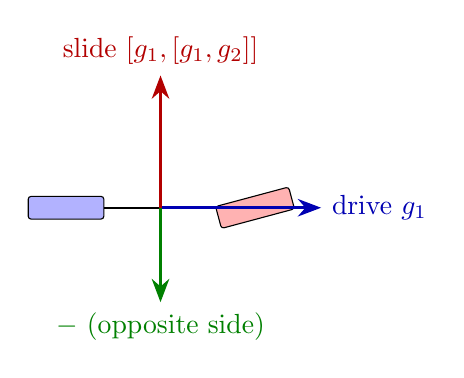
\begin{tikzpicture}[>=Stealth,scale=1.2]
\coordinate (R) at (0,0);
\coordinate (F) at (2,0);
\draw[thick] (R)--(F);
\wheel{(R)}{0}{blue!30}
\wheel{(F)}{15}{red!30}
\draw[->,very thick,blue!70!black] (1,0)--(2.7,0) node[right]{drive $g_1$};
\draw[->,very thick,red!70!black] (1,0)--(1,1.4) node[above]{slide $\LB{g_1}{\LB{g_1}{g_2}}$};
\draw[->,very thick,green!50!black] (1,0)--(1,-1.0) node[below]{$-$ (opposite side)};
\end{tikzpicture}
\caption{Bicycle at $\theta=0$: the second-order bracket $\LB{g_1}{\LB{g_1}{g_2}}\propto(-\sin\theta,\cos\theta,0,0)$ is the \emph{sliding} direction, perpendicular to the heading.}
\end{figure}

\begin{intuition}
The picture is the same as for the unicycle but one level deeper: \emph{steering} the wheel changes the \emph{turning rate} (first bracket, $\partial_\phi\dot\theta$ direction: a pure rotation of the body), and driving while rotating then produces a net \emph{sideways slide} (second-order bracket, with magnitude growing as $1/\cos^2\phi$). This is the car's parallel-parking motion. Four independent directions (drive, steer, rotate, slide) cover the four-dimensional state space.
\end{intuition}

% =====================================================================
\section{Summary}

\subsection{Comparison of the models}

\begin{table}[ht]
\centering
\footnotesize
\setlength{\tabcolsep}{4pt}
\renewcommand{\arraystretch}{1.35}
\begin{tabular}{@{}p{2.6cm}p{3.0cm}p{3.7cm}p{4.3cm}@{}}
\toprule
 & \textbf{Unicycle} & \textbf{Bicycle RWD} & \textbf{Bicycle FWD}\\
\midrule
State $q$ ($n$) & $(x,y,\theta)$ ($3$) & $(x,y,\theta,\phi)$ ($4$) & $(x,y,\theta,\phi)$ ($4$)\\
Constraints $k$ / inputs $m$ & $1$ / $2$ & $2$ / $2$ & $2$ / $2$\\
Drive field $g_1$ & $(\cos\theta,\sin\theta,0)$ & $(\cos\theta,\sin\theta,\tfrac{\tan\phi}\ell,0)$ & $(\cos\theta\cos\phi,\sin\theta\cos\phi,\tfrac{\sin\phi}\ell,0)$\\
Steer field $g_2$ & $(0,0,1)$ & $(0,0,0,1)$ & $(0,0,0,1)$\\
Drive input $u_1$ & body speed $v$ & rear-wheel speed & front-wheel speed\\
Singularity & none & $\phi=\pm\pi/2$ & none\\
Brackets needed & $\LB{g_1}{g_2}$ & up to $\LB{g_1}{\LB{g_1}{g_2}}$ & same\\
Rank / controllable & $3=n$, yes & $4=n$, yes & $4=n$, yes\\
\bottomrule
\end{tabular}
\caption{Kinematic models and their controllability.}
\end{table}

\begin{figure}[H]
\centering
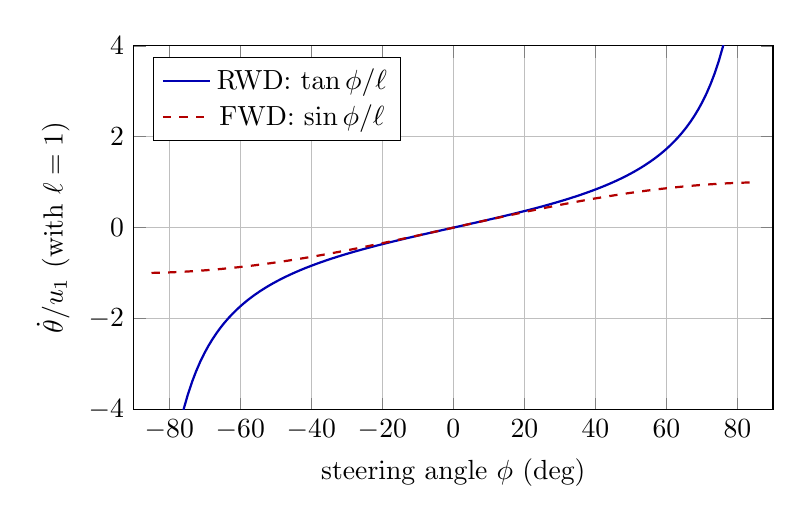
\begin{tikzpicture}
\begin{axis}[width=0.8\textwidth,height=6.2cm,xlabel={steering angle $\phi$ (deg)},
 ylabel={$\dot\theta/u_1$ (with $\ell=1$)},domain=-85:85,samples=150,
 ymin=-4,ymax=4,xmin=-90,xmax=90,grid=major,legend pos=north west,unbounded coords=jump]
\addplot[thick,blue!70!black] {tan(x)};
\addplot[thick,red!70!black,dashed] {sin(x)};
\legend{RWD: $\tan\phi/\ell$,FWD: $\sin\phi/\ell$}
\end{axis}
\end{tikzpicture}
\caption{Rotation rate per unit of drive speed: it blows up at $\phi=\pm\pi/2$ for the rear-wheel-drive model but stays bounded for the front-wheel-drive one.}
\end{figure}

\subsection{Key take-aways}

\begin{itemize}
\item The bicycle has $n=4$ coordinates and $2$ independent pure-rolling constraints: the null space has dimension $2$, giving the drive and steer vector fields. RWD uses $g_1=(\cos\theta,\sin\theta,\tan\phi/\ell,0)$ and is singular at $\phi=\pi/2$; FWD uses $g_1\cos\phi$ and has no singularity.
\item Controllability of driftless nonlinear systems is about \emph{directions}: the Lie bracket $\LB{g_1}{g_2}=\frac{\partial g_2}{\partial x}g_1-\frac{\partial g_1}{\partial x}g_2$ gives new directions, and the four-leg manoeuvre displaces the state by $\varepsilon^2\LB{g_1}{g_2}+O(\varepsilon^3)$.
\item Chow's theorem (Lie algebra / accessibility rank condition): the system is controllable iff the accessibility distribution generated by $g_i$ and all iterated brackets has dimension $n$.
\item Unicycle: $\LB{g_1}{g_2}=(\sin\theta,-\cos\theta,0)$ is the forbidden sliding direction, so rank $3$ and it is controllable. Bicycle: $\LB{g_1}{g_2}$ and $\LB{g_1}{\LB{g_1}{g_2}}$ supply the missing rotation and slide, rank $4$, hence controllable.
\item Controllability with fewer inputs than states is equivalent to the kinematic constraints being non-integrable, i.e.\ nonholonomic.
\end{itemize}

\end{document}